\section{CORAL 实验}

\begin{frame}{Deep CORAL 原实验复现}
\centering
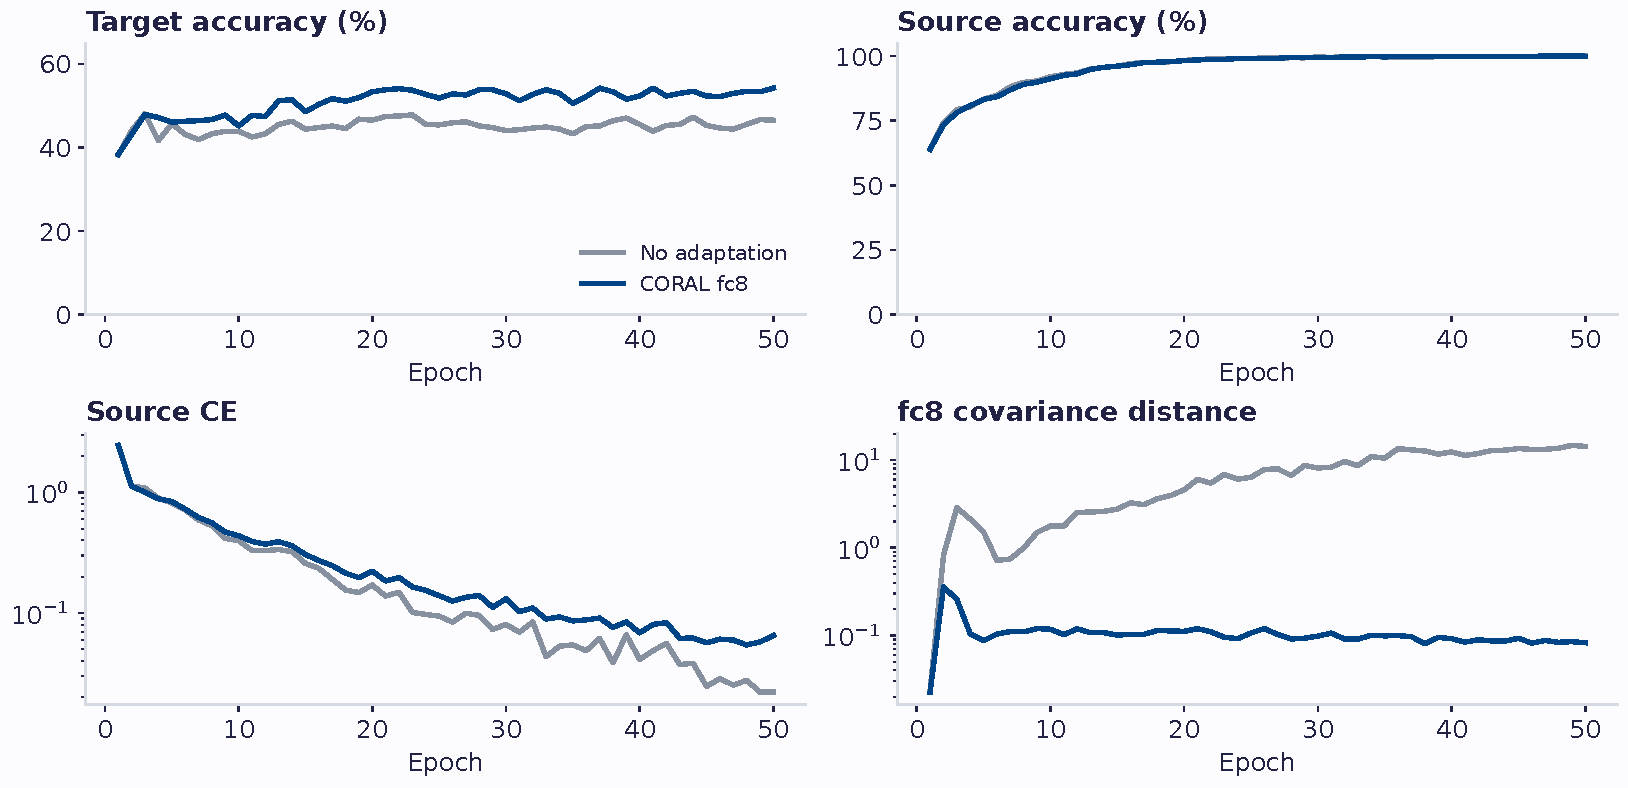
\includegraphics[width=\linewidth,height=.82\textheight,keepaspectratio]{baseline.pdf}
\end{frame}

\begin{frame}[t]{多层 CORAL 联合对齐}
\small
\[
\mathcal L=\CE+\frac{\lambda}{|\mathcal A|}\sum_{\ell\in\mathcal A}
\frac{\norm{C_s^{(\ell)}-C_t^{(\ell)}}_F^2}{4D_\ell^2},\qquad\lambda=0.5.
\]
\begin{tabularx}{\linewidth}{@{}lYY@{}}
\toprule
层 & 对齐对象 & 实际损失系数 \\
\midrule
conv5 & 空间位置上的 256 维通道特征 & 单层：0.5 \\
fc6 / fc7 & 4,096 维 Linear 输出，ReLU 前 & 双层：各 0.25 \\
fc8 & 31 维分类 logits & 三层：各 $1/6$ \\
\bottomrule
\end{tabularx}
\vspace{3mm}
\begin{itemize}
  \item 单层：conv5、fc6、fc7、fc8。
  \item 联合：conv5+fc8、fc6+fc7、fc6+fc8、fc7+fc8、fc6+fc7+fc8。
  \item AlexNet V1，Amazon$\to$Webcam，seed=42，batch=128，固定 50 轮。
\end{itemize}
\src{reports/data/layer\_results.csv；多层损失取均值。}
\end{frame}

\begin{frame}[t]{多层 CORAL：conv5+fc8 的正确率最高}
\fullfig{alex_layers.pdf}
\takeaway{conv5+fc8：55.09\%；fc8：54.21\%；无适应：46.54\%。更多对齐层没有带来单调改善。}
\src{AlexNet 位置实验，第 50 轮目标正确率。}
\end{frame}

\begin{frame}[t]{自适应 $\lambda$：梯度范数平衡}
\small
在共享 conv5 参数上计算梯度范数，EMA decay=0.9；$\lambda=e^s$：
\[
g_{\rm CE}=\norm{\nabla\CE}_2,\quad g_{\rm G}=\norm{\nabla\G}_2,\quad
\boxed{J_\lambda=(\lambda\overline g_{\rm G}-\overline g_{\rm CE})^2}.
\]
独立 Adam（lr=0.01）学习 $s$；模型更新时将 $\lambda$ detach。
\vspace{2mm}
\begin{tabularx}{\linewidth}{@{}Yrrr@{}}
\toprule
配置 & 最佳正确率 & 最终正确率 & 最终 $\lambda$ \\
\midrule
\LambdaRows
\bottomrule
\end{tabularx}
\takeaway{全程自适应 fc8 的最终正确率下降；联合组的峰值也没有提高。}
\src{reports/data/lambda\_results.csv；fc8 为 50 轮，conv5+fc8 为 100 轮。}
\end{frame}

\begin{frame}[t]{启用自适应后：$\lambda$ 激增，CORAL loss 快速下降}
\smallfig[.51]{lambda_failure.pdf}
\small
\begin{itemize}
  \item 第 50 轮启用后：$\lambda$ 从 0.5 升至 \textbf{6.94}；原始 $\G$ 从 0.0853 降至 \textbf{0.0167}。
  \item 出现 $\G\to0$ 的趋势，与论文强调避免的退化方向一致；对齐值下降未改善最佳正确率。
\end{itemize}
\takeaway{该自适应方案无效，依然采用固定 $\lambda=0.5$。}
\src{conv5+fc8 逐轮日志；\href{https://arxiv.org/pdf/1607.01719}{Deep CORAL \S3.2} 强调分类与对齐约束的平衡。}
\end{frame}

\begin{frame}[t]{停止条件：分类损失与加权 CORAL 损失平衡}
\small
记每轮训练均值 $a_e=\CE$、$b_e=0.5\G$，分别维护 decay=0.5 的 EMA。
\[
\delta(a,b)=\frac{|a-b|}{\max(a,b,10^{-12})}.
\]
\begin{block}{规则与条件}
从第 20 轮起，\textbf{当轮与 EMA 的相对差距均 $\le25\%$}，\textbf{连续两轮}满足则停止；最大预算 100 轮。
\end{block}
\vspace{1mm}
\textbf{设计目的：}保持固定适应强度，以训练内信号判断两项约束是否达到平衡，减少过长训练。
\par\vspace{3mm}
\textbf{conv5+fc8 结果：}日志回放在第 \textbf{58} 轮触发，正确率 \textbf{56.48\%}；第 100 轮为 52.58\%。原始 / EMA 差距分别为 13.17\% / 15.72\%。
\src{reports/data/early\_stop\_results.csv；停止信号只读取训练损失。}
\end{frame}

\begin{frame}[t]{ResNet-50：CORAL 的额外收益不明显}
\small
ImageNet V2，batch=32，共享 BN；$\lambda=0.5$，双层各 0.25；使用相同停止规则。
\vspace{2mm}
\begin{tabularx}{\linewidth}{@{}Yrrrr@{}}
\toprule
配置 & 停止轮 & 正确率 & 同轮对照正确率 & 同轮增益 \\
\midrule
\ResnetRows
\bottomrule
\end{tabularx}
\vspace{2mm}
无 CORAL 已达到 \textbf{80.00\%}；单独 pooled / layer4 对齐基本没有改善，含 logits 的配置有小幅收益。
\takeaway{在这种更先进的预训练网络上，CORAL 并未带来明显的性能跃迁。}
\src{reports/resnet50/summary.csv；同轮对照采用一致的共享 BN 配置。}
\end{frame}
